\documentclass[a4paper]{article}

\usepackage{pgfplots}

\pgfplotsset{compat=1.7}

\begin{document}

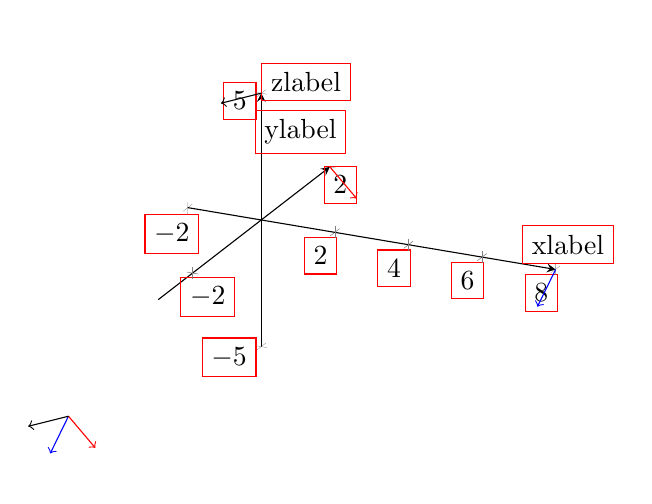
\begin{tikzpicture}
%\tracingcommands=2\tracingmacros=2
	\begin{axis}[axis lines=center,
		xmin=-2,xmax=8,
		ymin=-3,
		ymax=2,
		zmin=-5,
		zmax=5,
		xlabel=xlabel,
		ylabel=ylabel,
		zlabel=zlabel,
		show outer normals,
		xlabel style={at={(ticklabel* cs:1)}, anchor=near ticklabel opposite,draw=red},
		ylabel style={at={(ticklabel* cs:1)}, anchor=near ticklabel opposite,draw=red},
		zlabel style={at={(ticklabel* cs:1)}, anchor=near ticklabel opposite,draw=red},
		xticklabel style={draw=red},
		yticklabel style={draw=red},
		zticklabel style={draw=red},
	]
	
	\end{axis}
\end{tikzpicture}
\end{document}

